\section{Tutorial: A Picture for Karl's Students}

\subsection{Overview}
The expected outcome of this tutorial:
\begin{figure}[H]
    \includegraphics[width=1\textwidth]{a_picture_for_karls_students/figures/overview.PNG}
    \caption{Expected outcome but in Tikz.}
\end{figure}

\newpage
\subsection{Execution}

\begin{tikzpicture}
    \draw (-1.5,0) -- (1.5,0);
    \draw (0,-1.5) -- (0,1.5);
\end{tikzpicture}

\vspace{1cm}

\tikz \draw (-1.5,0) -- (1.5,0) -- (0,-1.5) -- (0,1.5);

\vspace{1cm}

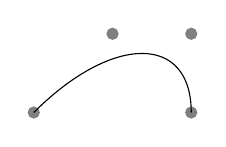
\begin{tikzpicture}
    \filldraw [gray] (0, 0) circle (2pt)
                     (1, 1) circle (2pt)
                     (2, 1) circle (2pt)
                     (2, 0) circle (2pt);
    \draw (0,0) .. controls (1,1) and (2,1) .. (2,0);
\end{tikzpicture}

\vspace{1cm}

\begin{tikzpicture}
    \draw (-1.5,0) -- (1.5,0);
    \draw (0,-1.5) -- (0,1.5);
    \draw (-1,0) .. controls (-1,0.555) and (-0.555,1) .. (0,1)
                 .. controls (0.555,1) and (1,0.555) .. (1,0);
\end{tikzpicture}

\vspace{1cm}

\tikz \draw (0,0) circle (10pt);

\vspace{1cm}

\tikz \draw (0,0) ellipse (20pt and 10pt);

\vspace{1cm}

\tikz \draw[rotate=30] (0,0) ellipse (20pt and 10pt);

\vspace{1cm}

\begin{tikzpicture}
    \draw (-1.5,0) -- (1.5,0);
    \draw (0,-1.5) -- (0,1.5);

    \draw (0,0) circle (1cm);
\end{tikzpicture}
 
\vspace{1cm}

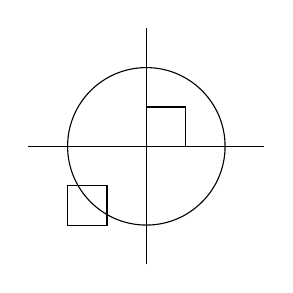
\begin{tikzpicture}
    \draw (-1.5,0) -- (1.5,0);
    \draw (0,-1.5) -- (0,1.5);
    \draw (0,0) circle (1cm);

    \draw (0,0) rectangle (0.5,0.5);
    \draw (-0.5,-0.5) rectangle (-1,-1);
\end{tikzpicture}

\vspace{1cm}

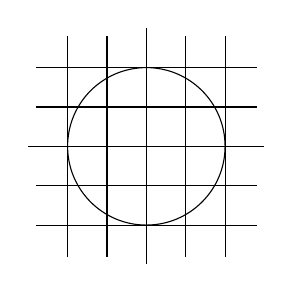
\begin{tikzpicture}
    \draw (-1.5,0) -- (1.5,0);
    \draw (0,-1.5) -- (0,1.5);
    \draw (0,0) circle (1cm);

    \draw[step=0.5cm] (-1.4,-1.4) grid (1.4,1.4);
\end{tikzpicture}

\vspace{1cm}

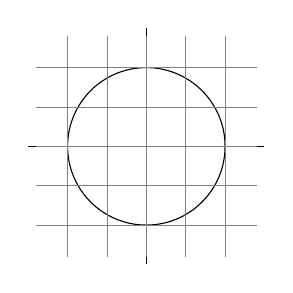
\begin{tikzpicture}
    \draw (-1.5,0) -- (1.5,0);
    \draw (0,-1.5) -- (0,1.5);
    \draw (0,0) circle (1cm);

    \draw[step=0.5cm,gray,very thin] (-1.4,-1.4) grid (1.4,1.4);
\end{tikzpicture}

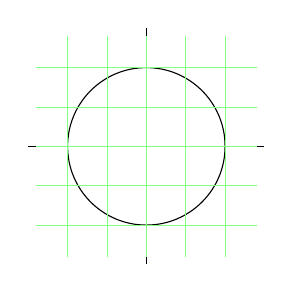
\begin{tikzpicture}
    \draw (-1.5,0) -- (1.5,0);
    \draw (0,-1.5) -- (0,1.5);
    \draw (0,0) circle (1cm);

    \draw[step=0.5cm,style=help lines] (-1.4,-1.4) grid (1.4,1.4);
\end{tikzpicture}

\tikzstyle{help lines} = [color=blue!50,very thin]

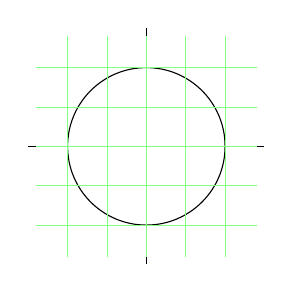
\begin{tikzpicture}
    \draw (-1.5,0) -- (1.5,0);
    \draw (0,-1.5) -- (0,1.5);
    \draw (0,0) circle (1cm);

    \draw[step=0.5cm,style=help lines] (-1.4,-1.4) grid (1.4,1.4);
\end{tikzpicture}

\tikzstyle{help lines} += [color=green!50]

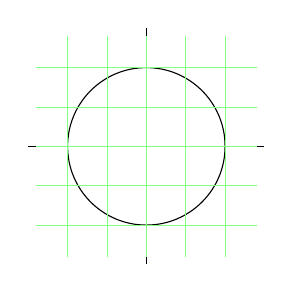
\begin{tikzpicture}
    \draw (-1.5,0) -- (1.5,0);
    \draw (0,-1.5) -- (0,1.5);
    \draw (0,0) circle (1cm);

    \draw[step=0.5cm,style=help lines] (-1.4,-1.4) grid (1.4,1.4);
\end{tikzpicture}

\tikzstyle{Karl's grid} = [style=help lines, color=blue!50]
\tikz \draw[style=Karl's grid] (0,0) grid (5,5);

\tikz \draw[Karl's grid] (0,0) grid (4,4);

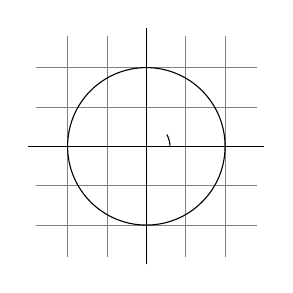
\begin{tikzpicture}
    \draw[step=0.5cm,gray,very thin] (-1.4,-1.4) grid (1.4,1.4);
    \draw (-1.5,0) -- (1.5,0);
    \draw (0,-1.5) -- (0,1.5);
    \draw (0,0) circle (1cm);
    
    \draw (3mm,0) arc (0:30:3mm);
\end{tikzpicture}

\vspace{1cm}

\begin{tikzpicture}[scale=3]
    \draw[step=0.5cm,gray,very thin] (-1.4,-1.4) grid (1.4,1.4);
    \draw (-1.5,0) -- (1.5,0);
    \draw (0,-1.5) -- (0,1.5);
    \draw (0,0) circle (1cm);
    
    \draw (3mm,0) arc (0:30:3mm);
\end{tikzpicture}

\tikz \draw (0,0) arc (0:315:1.75cm and 1cm);

\vspace{1cm}

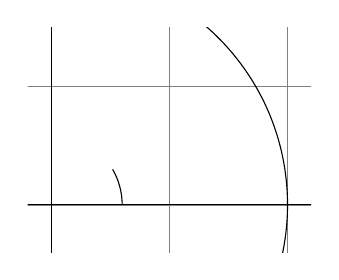
\begin{tikzpicture}[scale=3]
    \clip (-0.1,-0.2) rectangle (1.1,0.75);
    \draw[step=0.5cm,gray,very thin] (-1.4,-1.4) grid (1.4,1.4);
    \draw (-1.5,0) -- (1.5,0);
    \draw (0,-1.5) -- (0,1.5);
    \draw (0,0) circle (1cm);
    
    \draw (3mm,0) arc (0:30:3mm);
\end{tikzpicture}

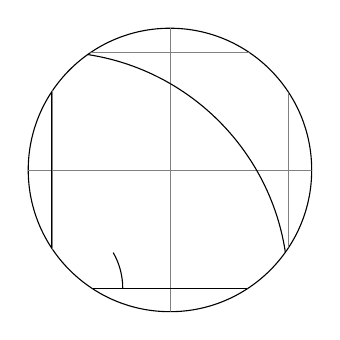
\begin{tikzpicture}[scale=3]
    \clip[draw] (0.5,0.5) circle (0.6cm);
    \draw[step=0.5cm,gray,very thin] (-1.4,-1.4) grid (1.4,1.4);
    \draw (-1.5,0) -- (1.5,0);
    \draw (0,-1.5) -- (0,1.5);
    \draw (0,0) circle (1cm);
    
    \draw (3mm,0) arc (0:30:3mm);
\end{tikzpicture}

\vspace{1cm}

\tikz \draw (0,0) rectangle (1,1)   (0,0) parabola (1,1);

\vspace{1cm}

\tikz \draw[x=1pt,y=1pt] (0,0) parabola bend (4,16) (6,12); % x=, y= is the length of the unit axes (standard 1cm each direction)

\vspace{1cm}

A sine \tikz \draw[x=1ex,y=1ex] (0,0) sin(1.57,1); curve.

A cos \tikz \draw[x=1ex,y=1ex] (0,0) cos(1.57,1); curve. 

\vspace{1cm}

\tikz \draw[x=1.57ex, y=1ex] (0,0) sin (1,1) cos (2,0) sin (3,-1) cos (4,0)
                             (0,1) cos (1,0) sin (2,-1) cos (3,0) sin (4,1);

\vspace{1cm}

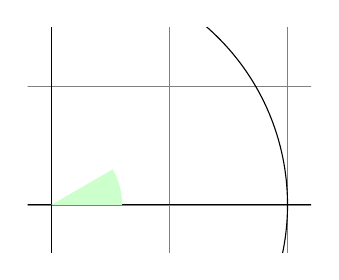
\begin{tikzpicture}[scale=3]
    \clip (-0.1,-0.2) rectangle (1.1,0.75);
    \draw[step=0.5cm,gray,very thin] (-1.4,-1.4) grid (1.4,1.4);
    \draw (-1.5,0) -- (1.5,0);
    \draw (0,-1.5) -- (0,1.5);
    \draw (0,0) circle (1cm);
    
    \fill[green!20!white] (0,0) -- (3mm,0) arc (0:30:3mm) -- (0,0);
\end{tikzpicture}

\vspace{1cm}


\begin{tikzpicture}[line width=5pt]
    \draw (0,0) -- (1,0) -- (1,1) -- (0,0);
    \draw (4,0) -- (5,0) -- (5,1) -- (4,1) -- (4,0);
    \draw (2,0) -- (3,0) -- (3,1) -- (2.5,1) -- cycle;
\end{tikzpicture}

\vspace{1cm}

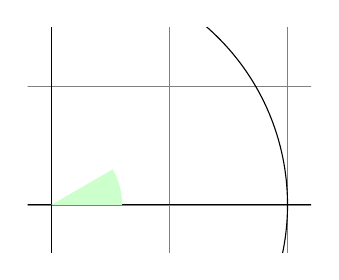
\begin{tikzpicture}[scale=3]
    \clip (-0.1,-0.2) rectangle (1.1,0.75);
    \draw[step=0.5cm,gray,very thin] (-1.4,-1.4) grid (1.4,1.4);
    \draw (-1.5,0) -- (1.5,0);
    \draw (0,-1.5) -- (0,1.5);
    \draw (0,0) circle (1cm);
    
    \fill[green!20!white] (0,0) -- (3mm,0) arc (0:30:3mm) -- cycle;
\end{tikzpicture}

\vspace{1cm}

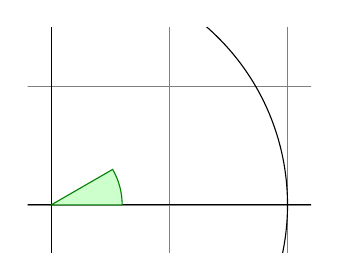
\begin{tikzpicture}[scale=3]
    \clip (-0.1,-0.2) rectangle (1.1,0.75);
    \draw[step=0.5cm,gray,very thin] (-1.4,-1.4) grid (1.4,1.4);
    \draw (-1.5,0) -- (1.5,0);
    \draw (0,-1.5) -- (0,1.5);
    \draw (0,0) circle (1cm);
    
    \filldraw[fill=green!20!white, draw=green!50!black] 
        (0,0) -- (3mm,0) arc (0:30:3mm) -- cycle;
\end{tikzpicture}

\vspace{1cm}

\tikz \shade (0,0) rectangle (2,1)   (3,0.5) circle (0.5cm);

\vspace{1cm}


\begin{tikzpicture}[rounded corners, ultra thick]
    \shade[top color=yellow, bottom color=black] (0,0) rectangle +(2,1);
    \shade[left color=yellow, right color=black] (3,0) rectangle +(2,1);
    \shadedraw[inner color=yellow, outer color=black, draw=red] (6,0) rectangle +(2,1);
    \shade[ball color=green] (9,0.5) circle (0.5cm);
\end{tikzpicture}

\vspace{1cm}

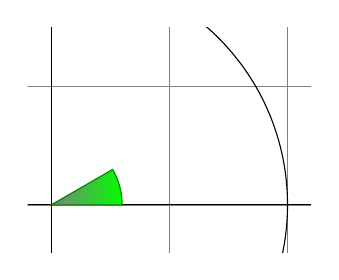
\begin{tikzpicture}[scale=3]
    \clip (-0.1,-0.2) rectangle (1.1,0.75);
    \draw[step=0.5cm,gray,very thin] (-1.4,-1.4) grid (1.4,1.4);
    \draw (-1.5,0) -- (1.5,0);
    \draw (0,-1.5) -- (0,1.5);
    \draw (0,0) circle (1cm);
    
    \shadedraw[left color=gray, right color=green, draw=green!50!black]
        (0,0) -- (3mm,0) arc (0:30:3mm) -- cycle;
\end{tikzpicture}

\vspace{1cm}

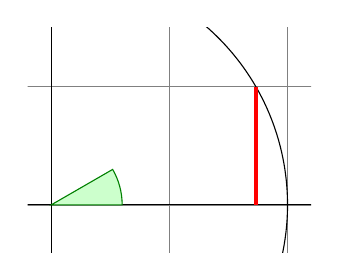
\begin{tikzpicture}[scale=3]
    \clip (-0.1,-0.2) rectangle (1.1,0.75);
    \draw[step=0.5cm,gray,very thin] (-1.4,-1.4) grid (1.4,1.4);
    \draw (-1.5,0) -- (1.5,0);
    \draw (0,-1.5) -- (0,1.5);
    \draw (0,0) circle (1cm);
    \filldraw[fill=green!20!white, draw=green!50!black] 
        (0,0) -- (3mm,0) arc (0:30:3mm) -- cycle;


    \draw[red,very thick] (30:1cm) -- +(0,-0.5);
    
\end{tikzpicture}

\vspace{1cm}

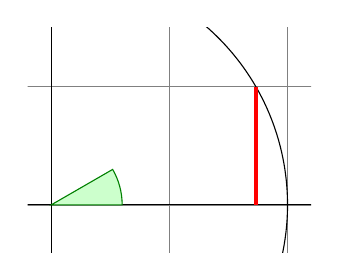
\begin{tikzpicture}[scale=3]
    \clip (-0.1,-0.2) rectangle (1.1,0.75);
    \draw[step=0.5cm,gray,very thin] (-1.4,-1.4) grid (1.4,1.4);
    \draw (-1.5,0) -- (1.5,0);
    \draw (0,-1.5) -- (0,1.5);
    \draw (0,0) circle (1cm);
    \filldraw[fill=green!20!white, draw=green!50!black] 
        (0,0) -- (3mm,0) arc (0:30:3mm) -- cycle;


    \draw[red,very thick] (30:1cm) -- (30:1cm |- 0,0); % (vert line |- horiz line) = intersection point
    
\end{tikzpicture}

\vspace{1cm}

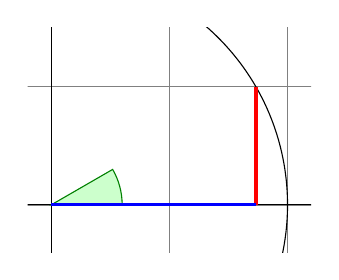
\begin{tikzpicture}[scale=3]
    \clip (-0.1,-0.2) rectangle (1.1,0.75);
    \draw[step=0.5cm,gray,very thin] (-1.4,-1.4) grid (1.4,1.4);
    \draw (-1.5,0) -- (1.5,0);
    \draw (0,-1.5) -- (0,1.5);
    \draw (0,0) circle (1cm);
    \filldraw[fill=green!20!white, draw=green!50!black] 
        (0,0) -- (3mm,0) arc (0:30:3mm) -- cycle;

    \draw[red,very thick] (30:1cm) -- +(0,-0.5);
    \draw[blue,very thick] (30:1cm) ++(0,-0.5) -- (0,0); % ++dist = distance from prev point
    
\end{tikzpicture}

\vspace{1cm}

% DOUBLE +
% Is relative the last given point
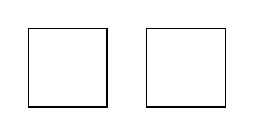
\begin{tikzpicture}
    \def\rectanglepath{-- ++(1cm,0cm) -- ++(0cm,1cm) -- ++(-1cm,0cm) -- cycle}
    \draw (0,0) \rectanglepath;
    \draw (1.5,0) \rectanglepath;
\end{tikzpicture}

\vspace{1cm}

% SINGLE +
% Is relative the first point given, here either (0,0) or (1.5,0)
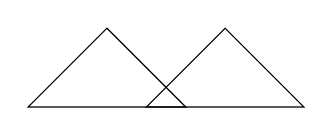
\begin{tikzpicture}
    \def\rectanglepath{-- +(1cm,0cm) -- +(0cm,1cm) -- +(-1cm,0cm) -- cycle}
    \draw (0,0) \rectanglepath;
    \draw (1.5,0) \rectanglepath;
\end{tikzpicture}

\vspace{1cm}

% SINGLE +
% Is relative the first point given, here either (0,0) or (1.5,0)
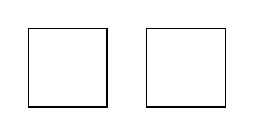
\begin{tikzpicture}
    \def\rectanglepath{-- +(1cm,0cm) -- +(1cm,1cm) -- +(0cm,1cm) -- cycle}
    \draw (0,0) \rectanglepath;
    \draw (1.5,0) \rectanglepath;
\end{tikzpicture}

\vspace{1cm}

% Same result but a better way
\tikz \draw (0,0) rectangle +(1,1)   (1.5,0) rectangle +(1,1);

\vspace{1cm}

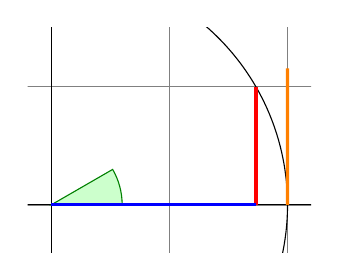
\begin{tikzpicture}[scale=3]
    \clip (-0.1,-0.2) rectangle (1.1,0.75);
    \draw[step=0.5cm,gray,very thin] (-1.4,-1.4) grid (1.4,1.4);
    \draw (-1.5,0) -- (1.5,0);
    \draw (0,-1.5) -- (0,1.5);
    \draw (0,0) circle (1cm);
    \filldraw[fill=green!20!white, draw=green!50!black] 
        (0,0) -- (3mm,0) arc (0:30:3mm) -- cycle;

    \draw[red,very thick] (30:1cm) -- +(0,-0.5);
    \draw[blue,very thick] (30:1cm) ++(0,-0.5) -- (0,0);
    
    % Intersection between lines that is not only vertical and horizontal
    % first infinite long line by two points 1,0--1,1
    % second infinite long line by two points 0,0--30:1cm
    \draw[orange,very thick] (1,0) -- (intersection of 1,0--1,1 and 0,0--30:1cm);
\end{tikzpicture}

\vspace{1cm}

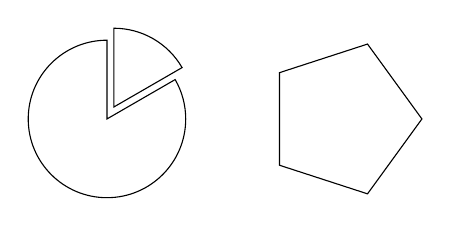
\begin{tikzpicture}
    \draw (0,0) -- (90:1cm) arc (90:360:1cm) arc (0:30:1cm) -- cycle;
    \draw (60:5pt) -- +(30:1cm) arc (30:90:1cm) -- cycle;

    \draw (3,0)     +(0:1cm) -- +(72:1cm) -- +(144:1cm) -- +(216:1cm) -- +(288:1cm) -- cycle;
\end{tikzpicture}

\vspace{1cm}

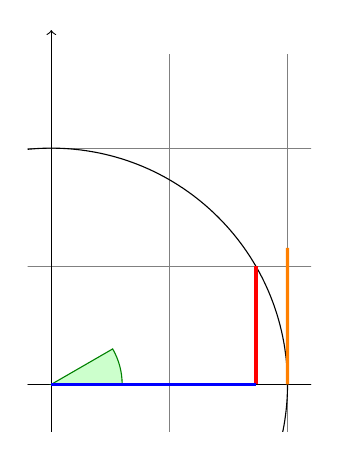
\begin{tikzpicture}[scale=3]
    \clip (-0.1,-0.2) rectangle (1.1,1.51);
    \draw[step=0.5cm,gray,very thin] (-1.4,-1.4) grid (1.4,1.4);
    \draw[->] (-1.5,0) -- (1.5,0);
    \draw[->] (0,-1.5) -- (0,1.5);
    \draw (0,0) circle (1cm);
    \filldraw[fill=green!20!white, draw=green!50!black] 
        (0,0) -- (3mm,0) arc (0:30:3mm) -- cycle;

    \draw[red,very thick] (30:1cm) -- +(0,-0.5);
    \draw[blue,very thick] (30:1cm) ++(0,-0.5) -- (0,0); 
    
    \draw[orange,very thick] (1,0) -- (intersection of 1,0--1,1 and 0,0--30:1cm);
\end{tikzpicture}

\vspace{1cm}

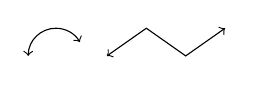
\begin{tikzpicture}
    \draw[<->] (0,0) arc (180:30:10pt);
    \draw[<->] (1,0) -- (1.5cm,10pt) -- (2cm,0pt) -- (2.5cm,10pt);
\end{tikzpicture}

\vspace{1cm}

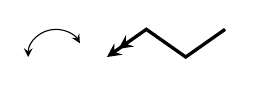
\begin{tikzpicture}[>=stealth] % arrow type = stealth plane look
    \draw[<->] (0,0) arc (180:30:10pt);
    \draw[<<-,very thick] (1,0) -- (1.5cm,10pt) -- (2cm,0pt) -- (2.5cm,10pt);
\end{tikzpicture}

\vspace{1cm}

\begin{tikzpicture}[ultra thick, red]
    \draw (0,0) -- (0,1);

    \begin{scope}[thin]
        \draw (1,0) -- (1,1);
        \draw (2,0) -- (2,1);
    \end{scope}

    \draw (3,0) -- (3,1);
\end{tikzpicture}

\vspace{1cm}

\tikz \draw (0,0) -- (0,0.5) [xshift=2pt] (0,0) -- (0,0.5); % Coordinate system transformation

\vspace{1cm}

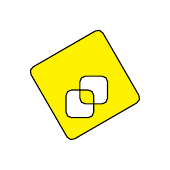
\begin{tikzpicture}[even odd rule, rounded corners=2pt, x=10pt, y=10pt]
    \filldraw[fill=yellow]          (0,0) rectangle (1,1)
        [xshift=5pt, yshift=5pt]    (0,0) rectangle (1,1)
        [rotate=30]                 (-1,-1) rectangle (2,2);
\end{tikzpicture}

\vspace{1cm}

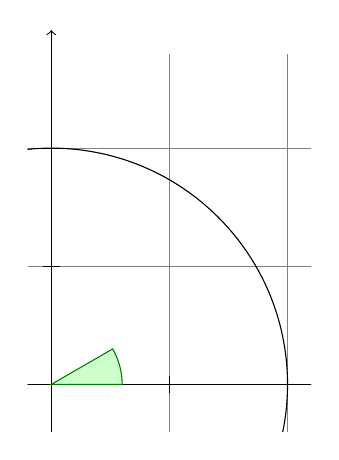
\begin{tikzpicture}[scale=3]
    \clip (-0.1,-0.2) rectangle (1.1,1.51);
    \draw[step=0.5cm,gray,very thin] (-1.4,-1.4) grid (1.4,1.4);

    \draw[->] (-1.5,0) -- (1.5,0);
    \draw[->] (0,-1.5) -- (0,1.5);

    \draw (0,0) circle (1cm);
    \filldraw[fill=green!20!white, draw=green!50!black] 
        (0,0) -- (3mm,0) arc (0:30:3mm) -- cycle;

    %\draw[red,very thick] (30:1cm) -- +(0,-0.5);
    %\draw[blue,very thick] (30:1cm) ++(0,-0.5) -- (0,0); 
    %\draw[orange,very thick] (1,0) -- (intersection of 1,0--1,1 and 0,0--30:1cm);

    \foreach \x in {-1cm,-0.5cm,0.5cm,1cm}
    {
        \draw (\x,-1pt) -- (\x,1pt);
    }
    \foreach \y in {-1cm,-0.5cm,0.5cm,1cm}
    {
        \draw (-1pt,\y) -- (1pt,\y);
    }

\end{tikzpicture}

\vspace{1cm}

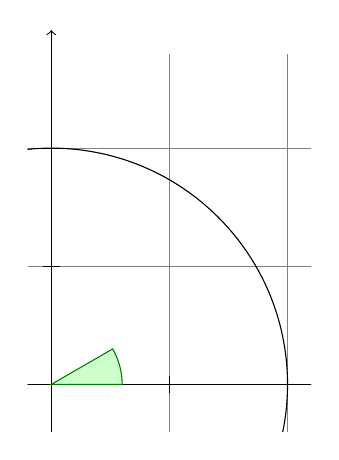
\begin{tikzpicture}[scale=3]
    \clip (-0.1,-0.2) rectangle (1.1,1.51);
    \draw[step=0.5cm,gray,very thin] (-1.4,-1.4) grid (1.4,1.4);

    \draw[->] (-1.5,0) -- (1.5,0);
    \draw[->] (0,-1.5) -- (0,1.5);

    \draw (0,0) circle (1cm);
    \filldraw[fill=green!20!white, draw=green!50!black] 
        (0,0) -- (3mm,0) arc (0:30:3mm) -- cycle;

    %\draw[red,very thick] (30:1cm) -- +(0,-0.5);
    %\draw[blue,very thick] (30:1cm) ++(0,-0.5) -- (0,0); 
    %\draw[orange,very thick] (1,0) -- (intersection of 1,0--1,1 and 0,0--30:1cm);

    % Same as previous
    \foreach \x in {-1,-0.5,0.5,1}
    {
        \draw[xshift=\x cm] (0,-1pt) -- (0,1pt);
    }
    \foreach \y in {-1cm,-0.5cm,0.5cm,1cm}
    {
        \draw[yshift=\y] (-1pt,0) -- (1pt,0);
    }

\end{tikzpicture}

\vspace{1cm}

\tikz   \foreach \x in {1,...,10} % OBS dimensionless
        {
            \draw (\x cm,0) circle (0.4cm);
        };

\vspace{1cm}

\tikz   \foreach \x in {-1,-0.5,...,1}
        {
            \draw (\x cm, -1pt) -- (\x cm, 1pt);
        };

\vspace{1cm}

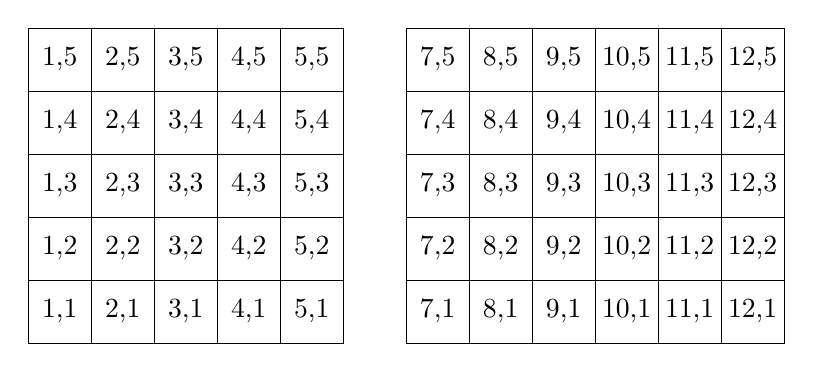
\begin{tikzpicture}[scale=0.8]
    \foreach \x in {1,2,...,5,7,8,...,12}
        \foreach \y in {1,...,5}
        {
            \draw (\x,\y) +(-.5,-.5) rectangle +(.5,.5);
            \draw (\x,\y) node{\x,\y};
        }
\end{tikzpicture}

\vspace{1cm}

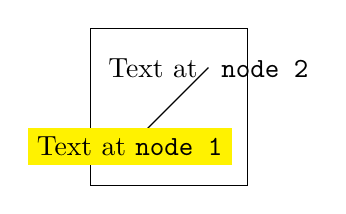
\begin{tikzpicture}
    \draw (0,0) rectangle (2,2);
    \draw   (0.5,0.5) node [fill=yellow] {Text at \verb!node 1!}
        --  (1.5,1.5) node {Text at \verb! node 2!};
\end{tikzpicture}

\vspace{1cm}

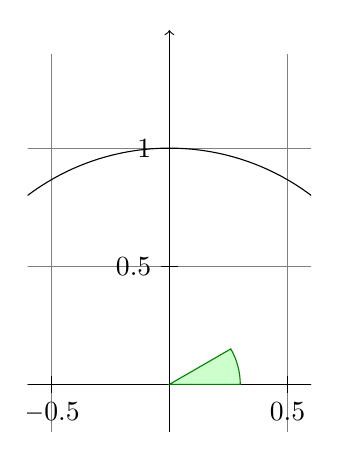
\begin{tikzpicture}[scale=3]
    \clip (-0.6,-0.2) rectangle (0.6,1.51);
    \draw[step=0.5cm,gray,very thin] (-1.4,-1.4) grid (1.4,1.4);

    \draw[->] (-1.5,0) -- (1.5,0);
    \draw[->] (0,-1.5) -- (0,1.5);

    \draw (0,0) circle (1cm);
    \filldraw[fill=green!20!white, draw=green!50!black] 
        (0,0) -- (3mm,0) arc (0:30:3mm) -- cycle;

    %\draw[red,very thick] (30:1cm) -- +(0,-0.5);
    %\draw[blue,very thick] (30:1cm) ++(0,-0.5) -- (0,0); 
    %\draw[orange,very thick] (1,0) -- (intersection of 1,0--1,1 and 0,0--30:1cm);

    % Same as previous
    \foreach \x in {-1,-0.5,0.5,1}
    {
        \draw[xshift=\x cm] (0,1pt) -- (0,-1pt) node[anchor=north] {$\x$};
    }
    \foreach \y in {-1,-0.5,0.5,1}
    {
        \draw[yshift=\y cm] (1pt,0) -- (-1pt,0) node[anchor=east] {$\y$};
    }

\end{tikzpicture}

\vspace{1cm}

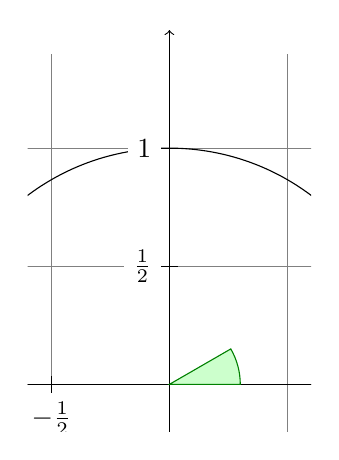
\begin{tikzpicture}[scale=3]
    \clip (-0.6,-0.2) rectangle (0.6,1.51);
    \draw[step=0.5cm,gray,very thin] (-1.4,-1.4) grid (1.4,1.4);

    \draw[->] (-1.5,0) -- (1.5,0);
    \draw[->] (0,-1.5) -- (0,1.5);

    \draw (0,0) circle (1cm);
    \filldraw[fill=green!20!white, draw=green!50!black] 
        (0,0) -- (3mm,0) arc (0:30:3mm) -- cycle;

    %\draw[red,very thick] (30:1cm) -- +(0,-0.5);
    %\draw[blue,very thick] (30:1cm) ++(0,-0.5) -- (0,0); 
    %\draw[orange,very thick] (1,0) -- (intersection of 1,0--1,1 and 0,0--30:1cm);

    % Two different variables, first used if second i absent (separated with /)
    \foreach \x / \xtext in {-1, -0.5/-\frac{1}{2}, 1}
    {
        \draw[xshift=\x cm] (0,1pt) -- (0,-1pt) node[anchor=north, fill=white] {$\xtext$};
    }
    \foreach \y / \ytext in {-1, -0.5/-\frac{1}{1}, 0.5/\frac{1}{2}, 1}
    {
        \draw[yshift=\y cm] (1pt,0) -- (-1pt,0) node[anchor=east, fill=white] {$\ytext$};
    }

\end{tikzpicture}

\vspace{1cm}

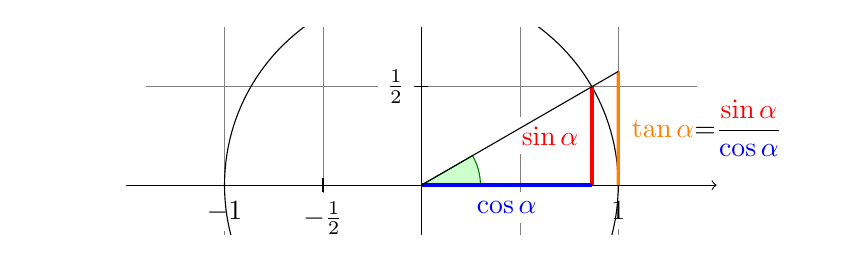
\begin{tikzpicture}[scale=2.5]
    \clip (-2,-.25) rectangle (2,0.8);
    \draw[step=0.5cm,gray,very thin] (-1.4,-1.4) grid (1.4,1.4);

    \draw[->] (-1.5,0) -- (1.5,0) coordinate(x axis);
    \draw[->] (0,-1.5) -- (0,1.5) coordinate(y axis);

    % Two different variables, first used if second i absent (separated with /)
    \foreach \x / \xtext in {-1, -0.5/-\frac{1}{2}, 1}
    {
        \draw[xshift=\x cm] (0,1pt) -- (0,-1pt) node[anchor=north, fill=white] {$\xtext$};
    }
    \foreach \y / \ytext in {-1, -0.5/-\frac{1}{1}, 0.5/\frac{1}{2}, 1}
    {
        \draw[yshift=\y cm] (1pt,0) -- (-1pt,0) node[anchor=east, fill=white] {$\ytext$};
    }

    \draw (0,0) circle (1cm);
    \filldraw[fill=green!20!white, draw=green!50!black] 
        (0,0) -- (3mm,0) arc (0:30:3mm) -- cycle;

    \draw[red,very thick] (30:1cm) -- node[left=1pt,fill=white]
        {$\sin\alpha$}
        (30:1cm |- x axis);
    \draw[blue,very thick] (30:1cm |- x axis) -- node[below=2pt,fill=white]
        {$\cos\alpha$}
        (0,0);
    \draw[orange,very thick] (1,0) -- node[right=1pt,fill=white]
        {$\displaystyle \tan\alpha \color{black}{=} \frac{\color{red}{\sin\alpha}}{\color{blue}{\cos\alpha}}$}
        (intersection of 1,0--1,1 and 0,0--30:1cm) coordinate(t);

    \draw (0,0) -- (t);
\end{tikzpicture}

\vspace{1cm}

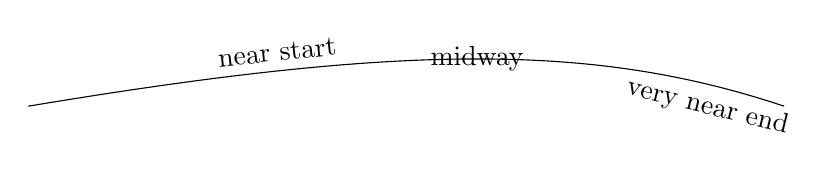
\begin{tikzpicture}[scale=0.8]
    \draw (0,0) .. controls (6,1) and (9,1) ..
        node[near start,sloped,above]{near start}
        node{midway}
        node[very near end,sloped,below]{very near end}
        (12,0);
\end{tikzpicture}

\vspace{1cm}

\begin{figure}
\centering
\makebox[0pt]{
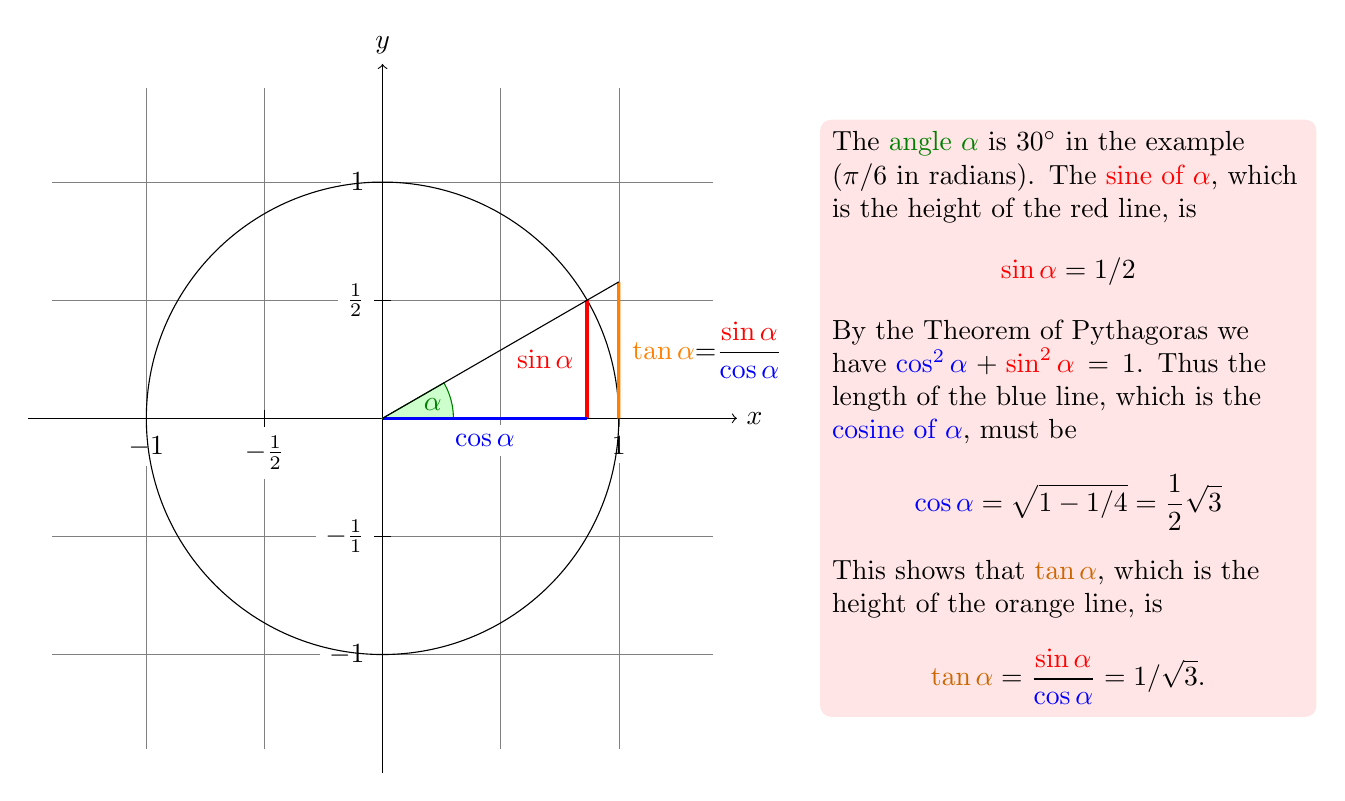
\begin{tikzpicture}[scale=3]
    % Local definitions
    \def\costhirty{0.8660256}
    
    % Styles
    \tikzstyle{information text} =  [rounded corners,fill=red!10,inner sep=1ex]
    \tikzstyle{important line} = [very thick]

    % Colors
    \colorlet{angle color}{green!50!black}
    \colorlet{sin color}{red}
    \colorlet{tan color}{orange!80!black}
    \colorlet{cos color}{blue}
    
    %%% Grid and axes
    \draw[step=0.5cm,gray,very thin] (-1.4,-1.4) grid (1.4,1.4);
    \draw[->] (-1.5,0) -- (1.5,0) node[right]{$x$} coordinate(x axis);
    \draw[->] (0,-1.5) -- (0,1.5) node[above]{$y$} coordinate(y axis);

    \foreach \x / \xtext in {-1, -0.5/-\frac{1}{2}, 1}
    {
        \draw[xshift=\x cm] (0,1pt) -- (0,-1pt) node[anchor=north, fill=white] {$\xtext$};
    }
    \foreach \y / \ytext in {-1, -0.5/-\frac{1}{1}, 0.5/\frac{1}{2}, 1}
    {
        \draw[yshift=\y cm] (1pt,0) -- (-1pt,0) node[anchor=east, fill=white] {$\ytext$};
    }
    %%%

    %%% Graphing
    \draw (0,0) circle (1cm);

    % Alpha angle
    \filldraw[fill=green!20!white, draw=green!50!black] 
        (0,0) -- (3mm,0) arc (0:30:3mm) -- cycle;
    \draw (15:2.2mm) node[angle color]{$\alpha$};

    % Marked lines
    \draw[red,important line] (30:1cm) -- node[left=1pt,fill=white]
        {$\sin\alpha$}
        (30:1cm |- x axis);
    \draw[blue,important line] (30:1cm |- x axis) -- node[below=2pt,fill=white]
        {$\cos\alpha$}
        (0,0); 
    \draw[orange,important line] (1,0) -- node[right=1pt,fill=white]
        {$\displaystyle \tan\alpha \color{black}{=} \frac{\color{red}{\sin\alpha}}{\color{blue}{\cos\alpha}}$}
        (intersection of 1,0--1,1 and 0,0--30:1cm) coordinate(t);

    \draw (0,0) -- (t);
    %%%
    
    %%% Text box
    \draw[xshift=1.85cm]
        node[right,text width=6cm,style=information text]
        {
            The {\color{angle color} angle $\alpha$} is $30^\circ$ in the example ($\pi/6$ in radians). 
            The {\color{sin color}sine of $\alpha$}, which is the height of the red line, is
            \[
                {\color{sin color}\sin\alpha} = 1/2    
            \]
            By the Theorem of Pythagoras we have ${\color{cos color}\cos^2\alpha} + {\color{sin color}\sin^2\alpha} = 1$. 
            Thus the length of the blue line, which is the {\color{cos color}cosine of $\alpha$}, must be
            \[
                {\color{cos color} \cos\alpha} = \sqrt{1 - 1/4} = \frac{1}{2}\sqrt{3}
            \]
            This shows that {\color{tan color} $\tan\alpha$}, which is the height of the orange line, is
            \[
                {\color{tan color}\tan\alpha} = \frac{{\color{sin color}\sin\alpha}}{{\color{cos color}\cos\alpha}} = 1/\sqrt{3}. 
            \]
        };
    %%%
\end{tikzpicture}
}
\end{figure}
